\clearpage\begingroup
\SourceLeaf{169}\HistoricalHead{164}{L}{PHYSIK.\quad BRIEFWECHSEL.}
\newcommand{\DioptrikLetterTwentyTwoDiagram}{%
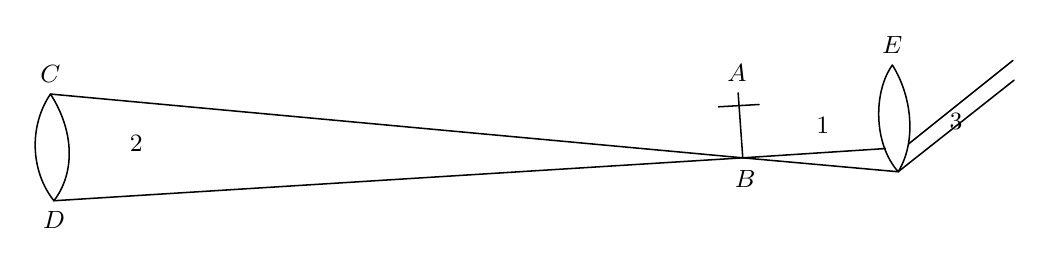
\begin{tikzpicture}[x=.0058in,y=-.0058in,line width=.55pt,line cap=round,line join=round]
\draw (39,63) .. controls (20,91) and (22,130) .. (42,155)
 .. controls (61,130) and (59,94) .. (39,63);
\draw (39,63) -- (636,118) -- (770,130) -- (870,51);
\draw (42,155) -- (636,118) -- (759,110);
\draw (779,106) -- (869,34);
\draw (765,38) .. controls (749,60) and (748,105) .. (770,130)
 .. controls (786,104) and (782,65) .. (765,38);
\draw (632,62) -- (636,118);
\draw (615,74) -- (650,72);
\node[anchor=south,font=\small] at (39,62) {$C$};
\node[anchor=north,font=\small] at (42,156) {$D$};
\node[anchor=south,font=\small] at (631,61) {$A$};
\node[anchor=north,font=\small] at (638,120) {$B$};
\node[anchor=south,font=\small] at (765,37) {$E$};
\node[font=\small] at (113,106) {$2$};
\node[font=\small] at (705,90) {$1$};
\node[font=\small] at (820,87) {$3$};
\end{tikzpicture}%
}

\begin{center}
[22.]\par\medskip
\textbf{\textsc{Gauss} an \textsc{Schumacher}.\quad Göttingen, 27. Junius 1846.}\par\medskip
\rule{.82\linewidth}{.4pt}\par\smallskip
{\footnotesize [Briefwechsel zwischen \textsc{Gauss} und \textsc{Schumacher} V, Altona 1863, S. 170.]}\par\smallskip
\rule{.82\linewidth}{.4pt}
\end{center}
\noindent . . . . . . . . . . . . . . . . . . . . .\par
\noindent\hspace*{\parindent}Ich will jedoch eine Bemerkung mittheilen, die sich mir bei Gelegenheit meines diesmaligen Vortrags dargeboten hat; ich habe zwar jetzt nicht Zeit gehabt in dem \textsc{Piper}schen Manuscript[*)]\begingroup\renewcommand{\thefootnote}{}\footnotetext{[*) Kollegienheft nach einer Vorlesung von \textsc{Gauss}.]}\endgroup\ die betreffende Stelle aufzusuchen, erinnere mich aber, dass Sie in einem früheren Briefe des Gegenstandes, als in dem Manuscript vorkommend, erwähnt haben.

Es ist der Satz, dass beim Gebrauch der Fernröhre der Kurzsichtige gegen den Weitsichtigen im Vortheil sei, weil er eine stärkere Vergrösserung geniesse. Sie bemerkten sehr richtig, dass die \textsc{Galilei}schen Fernröhre auszunehmen seien, wo das Gegentheil gelte, welche Fernröhre ich auch von meinem Vortrage von vorne herein ganz ausgeschlossen hatte. Aber die nähere Prüfung, die ich diesmal angestellt habe, zeigt, dass jener Satz auch bei astronomischen Fernröhren unrichtig, oder wenn Sie lieber wollen, dass er nur bedingungsweise richtig ist. Die Sache ist wirklich etwas captiös, und Ihnen daher vielleicht interessant, wenn ich etwas dabei verweile. Es ist ganz richtig, dass beim Betrachten eines \textls[120]{Objects} durch eine Loupe der Kurzsichtige im Vortheil vor dem Weitsichtigen ist, indem er mit der Loupe näher kommen kann und dadurch sich eine stärkere Vergrösserung verschafft. Bei dem astronomischen Fernrohr ist das Ocularglas eine Loupe, wodurch man das vom Objective dargestellte Bild betrachtet, und der Kurzsichtige bringt die Loupe dem Object (diesem Bilde) bekanntermaassen näher. Scheint daher meine frühere Behauptung nicht absolut richtig zu sein?

Sie ist es dennoch nicht.
\begin{center}\DioptrikLetterTwentyTwoDiagram\end{center}
\noindent\hspace*{\parindent}Es sei $CD$ das Objectiv, $AB$ das Bild eines Gegenstandes, $E$ das Ocular.
\par\clearpage\SourceLeaf{170}\HistoricalHead{165}{R}{GAUSS AN SCHUMACHER UND OLBERS.}
\noindent Ich sage nun, es ist nicht einerlei, ob $AB$ ein wirkliches Object ist, oder ein durch $CD$ effectuirtes Bild. Im ersten Fall schickt jeder Punkt von $AB$ z. B. \textls[120]{nach allen} Seiten Strahlen aus, im zweiten \textls[120]{bloss innerhalb} des kegelförmigen Raumes 1, der dieselbe Öffnung hat, wie der kegelförmige Raum $BCD=2$. Jene Strahlen füllen nach dem Durchgange durch $E$ einen beschränkten Raum 3 cylindrisch für weitsichtige Augen, conisch (eventuell herkommend von einer Spitze, für mich z. B. 5 Zoll entfernt) [für kurzsichtige], und da wo die Axe dieses Cylinders oder Kegels die Axe des Fernrohrs trifft, soll das Auge stehen, um alle Strahlen am besten aufzufangen. Man nennt das den Ort des Auges. Dieser Ort des Auges liegt nun (wie eine genauere Untersuchung zeigt) etwas weniges entfernter von dem Ocular bei der Stellung für ein kurzsichtiges Auge, als bei der für ein weitsichtiges, und durch diesen Umstand wird die grössere Annäherung des Oculars gegen das vom Object formirte Bild, die der Kurzsichtige anwendet, \textls[120]{mehr} als compensirt, so dass der Kurzsichtige, falls er sein Auge wirklich genau an den für sein Auge gültigen Ort bringt, allerdings eine~.etwas schwächere Vergrösserung hat, als der Fernsichtige. . . . . . . .
\clearpage\endgroup
